\documentclass[../ClassicThesis.tex]{subfiles}
\begin{document}

%************************************************
\chapter{Userinteraction}\label{ch:userinteraction}
%************************************************

%\note{design entscheidungen begründen?}

As our software is a converter, we minimized the required user interaction.

\section{Drag n Drop as Main Interaction}

Because the main function of our web service is converting custom objects, uploading a model is made easy by providing a drop area. This spread out over the whole web site. Alternatively we provide a upload button.

\section{The Landing Page combines Conversion Area with Repository}

The landing page is horizontally divided into two parts. At the top of the page is the conversion and preview area. Underneath this we show a repository of known \threedmodel s (see Figure~\ref{fig:landing_page}).

\begin{figure}
  \centering
  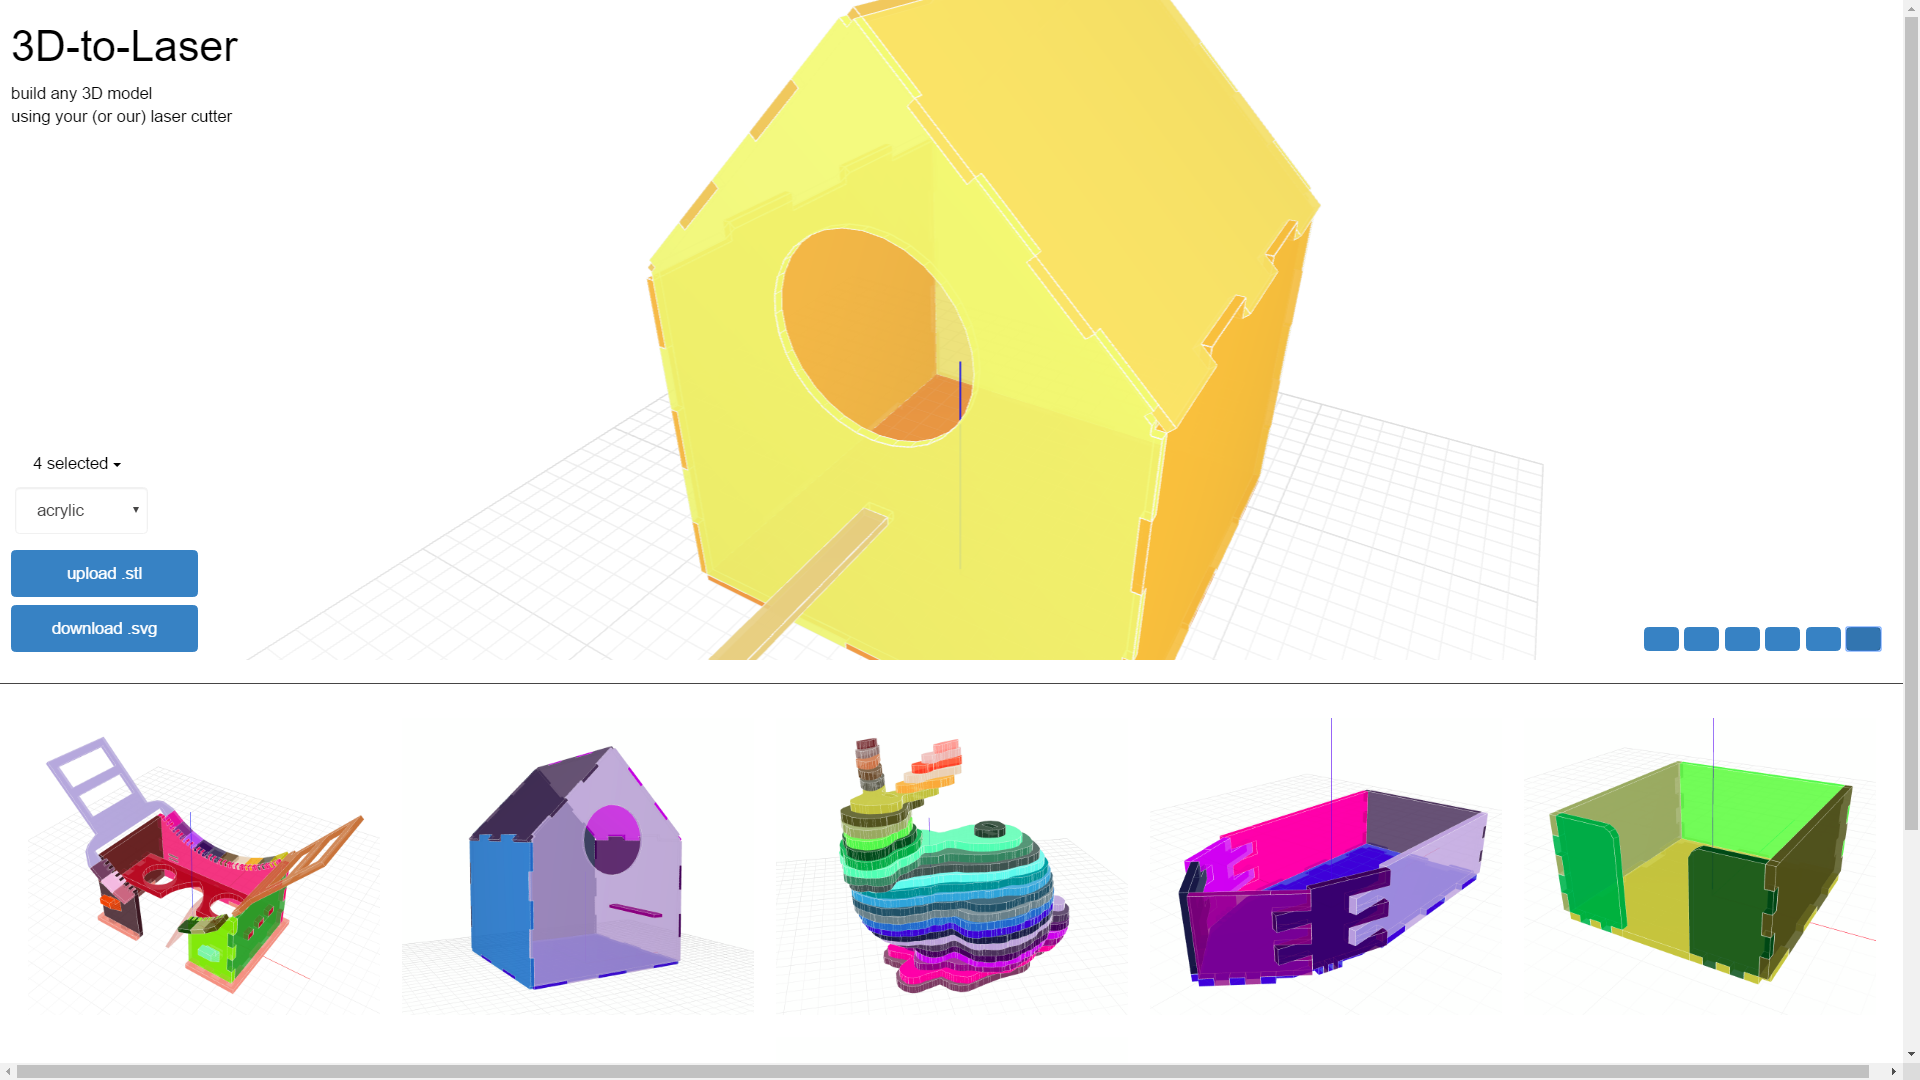
\includegraphics[width=1\columnwidth]{02-landing_page}
  \caption{The landing page with the conversion and the repository area.}
  \label{fig:landing_page}
\end{figure}

\subsection{The Conversion and Preview Area Provides the Main Functionality}

The conversion and preview area shows the currently selected or uploaded model. It also provides some conversion settings at the bottom left and a visualization selection at the bottom right.

\subsubsection{Conversion Settings for Custom Material Selection}

To change which materials should be used for the conversion, the user can select multiple plate thicknesses in the top selection drop down (see Figure~\ref{fig:thickness_select}). Additionally the drop down below provides the choice of the base material. Acrylic, wood, cardboard and paper are available yet (see Figure~\ref{fig:material_select}). The \emph{upload .stl} button adds a discoverable way of uploading an own model for conversion, unlike drag an drop as upload possibility.

\begin{figure}
    \centering
    \begin{subfigure}[t]{0.3\textwidth}
      \centering
      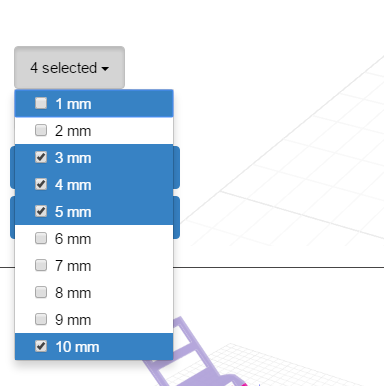
\includegraphics[width=\textwidth]{02-thickness_select}
      \caption{The thickness selection provides several options to choose from and combine.}
      \label{fig:thickness_select}
    \end{subfigure}
    \begin{subfigure}[t]{0.3\textwidth}
      \centering
      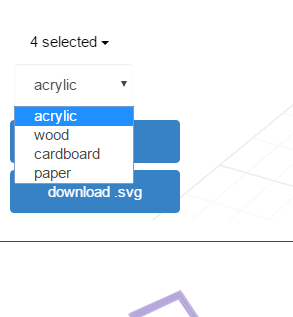
\includegraphics[width=\textwidth]{02-material_select}
      \caption{Currently this four materials are supported by our software.}
      \label{fig:material_select}
    \end{subfigure}
    \begin{subfigure}[t]{0.3\textwidth}
      \centering
      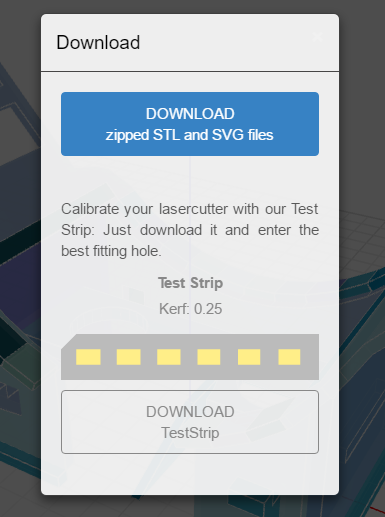
\includegraphics[width=\textwidth]{02-download_dialog}
      \caption{The download dialog also provides the possibility to calibrate the \svgfile{} to the used \lasercutter .}
      \label{fig:download_dialog}
    \end{subfigure}
    \caption{}
    \label{fig:conversion_settings}
\end{figure}

At the bottom we placed the \emph{download .svg} button. If the user clicks this, the download is not started directly. It opens the download dialog (see Figure~\ref{fig:download_dialog}).

%\note{make sure that the ui matches the functionality:}
The download dialog contains the \emph{DOWNLOAD zipped SVG files} button. This directly starts the download of the zipped result of the conversion, including one \svgfile{} for each used plate thickness. Underneath this the dialog shows a short explanation of the test strip (see \sectionref{sec:test_strip}) and an interactive test strip. It makes it possible to select the best fitting hole by clicking it. To create the corresponding strip the dialog provides also a download button for this.

\subsubsection{The Test Strip Enables Easy Kerf Error Reduction}
\label{sec:test_strip}

%\note{Image of test strip?}

The test strip is a small cutting plan with multiple rectangular holes and a small spike (see Figure~\ref{fig:test_strip}). The holes all have slightly different widths. The User can try in which hole the spike fits best. If he selects the corresponding hole in the user interface, our software calculates the kerf of the \lasercutter . This  makes it easy to determine the kerf without special equipment. We use the result for the calibration (see \sectionref{sec:calibration});

\begin{figure}
  \centering
  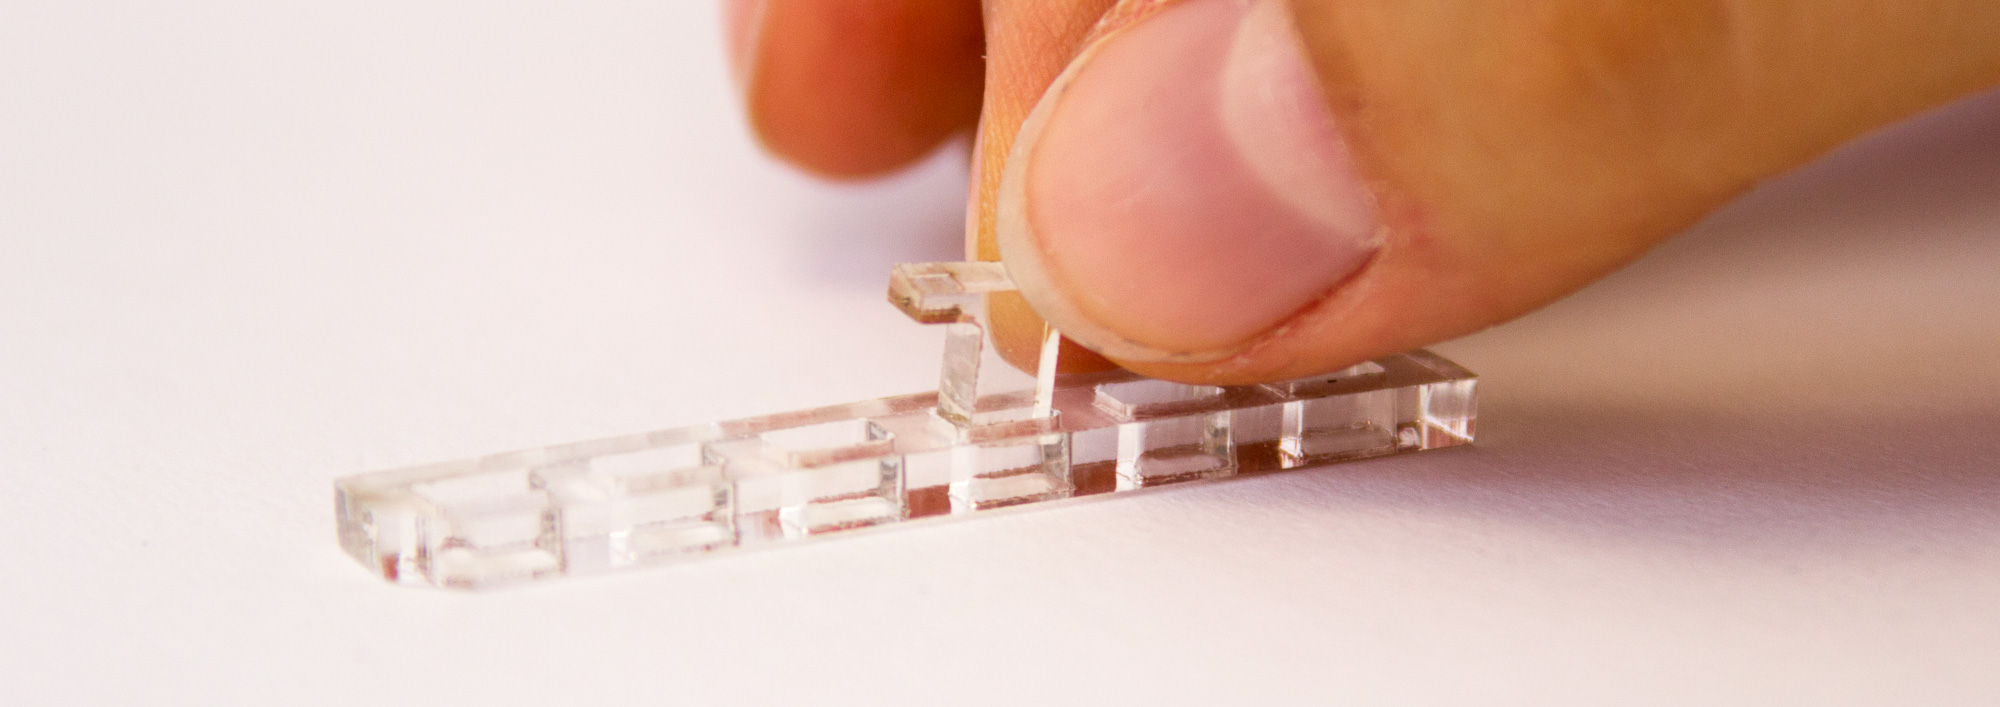
\includegraphics[width=1\columnwidth]{02-test_strip}
  \caption{The test strip with the spike.}
  \label{fig:test_strip}
\end{figure}

\subsubsection{The Visualizations Helps to Understand the Conversion}

The visualization selection contains six buttons where each of this activate another visualization. The selection includes in this order: the original .stl model, a wireframe view, a visualization of the coplanar faces, a view of the generated plates, a visualization of the plates with highlighted bend plates and one of the final model including the generated joints (see Figure~\ref{fig:visualization_selection}).

\begin{figure}
    \centering
    \begin{subfigure}[t]{0.49\textwidth}
      \centering
      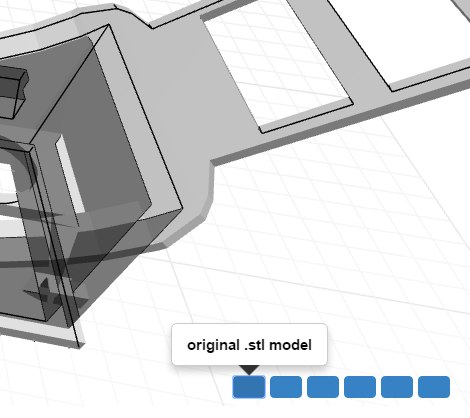
\includegraphics[width=\textwidth]{02-vis_model}
      \caption{The model visualization shows the original mesh.}
    \end{subfigure}
    \begin{subfigure}[t]{0.49\textwidth}
      \centering
      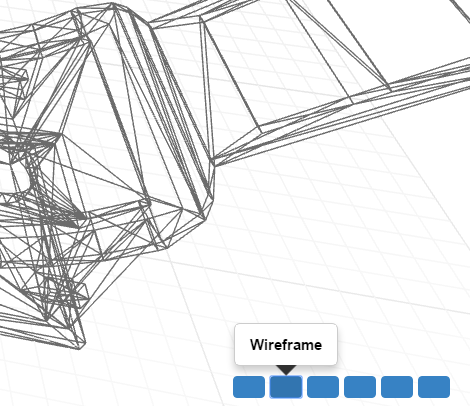
\includegraphics[width=\textwidth]{02-vis_wireframe}
      \caption{The wireframe visualization shows the triangles of the original mesh.}
    \end{subfigure}
    \begin{subfigure}[t]{0.49\textwidth}
      \centering
      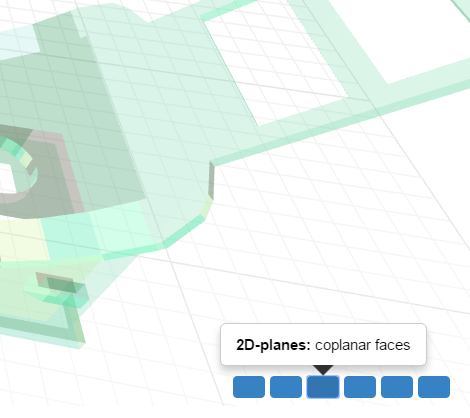
\includegraphics[width=\textwidth]{02-vis_coplanar}
      \caption{The coplanar visualization shows which faces create a flat surface.}
    \end{subfigure}
    \begin{subfigure}[t]{0.49\textwidth}
      \centering
      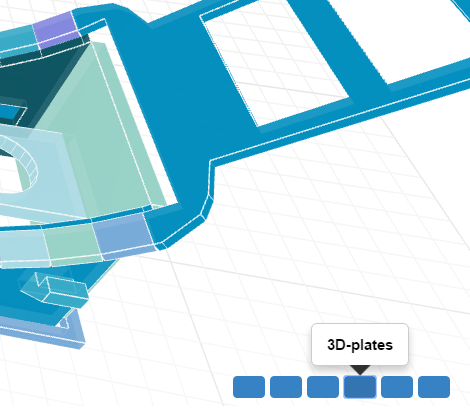
\includegraphics[width=\textwidth]{02-vis_plates}
      \caption{The plate visualization shows the generated plates.}
    \end{subfigure}
    \begin{subfigure}[t]{0.49\textwidth}
      \centering
      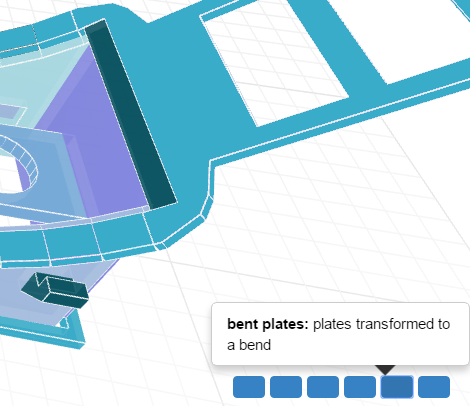
\includegraphics[width=\textwidth]{02-vis_bends+}
      \caption{The bend plate visualization uses for plates of the same bent plate the same color.}
    \end{subfigure}
    \begin{subfigure}[t]{0.49\textwidth}
      \centering
      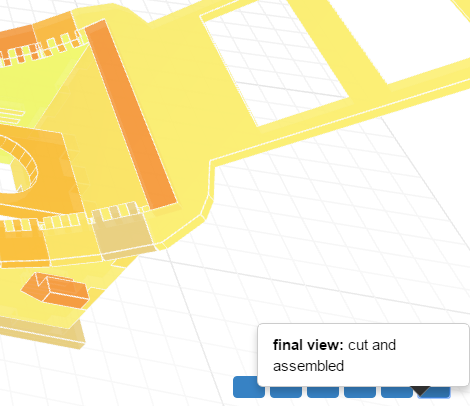
\includegraphics[width=\textwidth]{02-vis_joints}
      \caption{The final visualization shows all plates with the generated joints.}
    \end{subfigure}
    \caption{}
    \label{fig:visualization_selection}
\end{figure}

\subsection{The Repository Guarantees Fast Access to Lasercut-able Models}

The bottom part of the web page is a gallery of a repository of converted \threedmodel s. If the mouse hovers over one of the shown models, the gallery shows a overlay menu over this. This overlay includes the name of the model, a \emph{view} and a \emph{download .svg} button (see Figure~\ref{fig:gallery_overlay}).

\begin{figure}
  \centering
  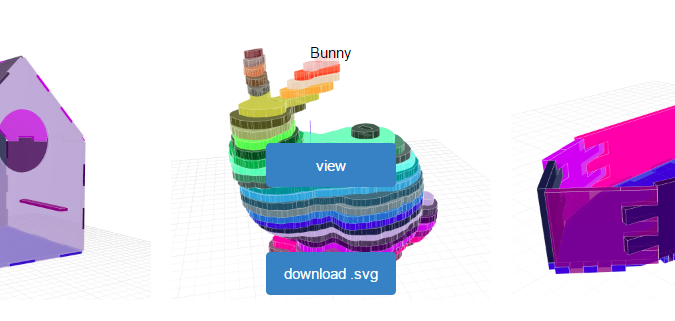
\includegraphics[width=1\columnwidth]{02-gallery_overlay}
  \caption{The hover menu in the gallery.}
  \label{fig:gallery_overlay}
\end{figure}

The \emph{view} button loads the selected model in the conversion area to show more details of the conversion and fine tuning it. The \emph{download .svg} button starts the download of the converted model directly.

\section{Debug View for more profound Conversion Analyses}

For detailed analyses of the conversion of an \threedmodel and single conversion steps the debug view can be used. It can be found at \url{localhost:3000/#/debug} (see Figure~\ref{fig:debug_view}).

\begin{figure}
  \centering
  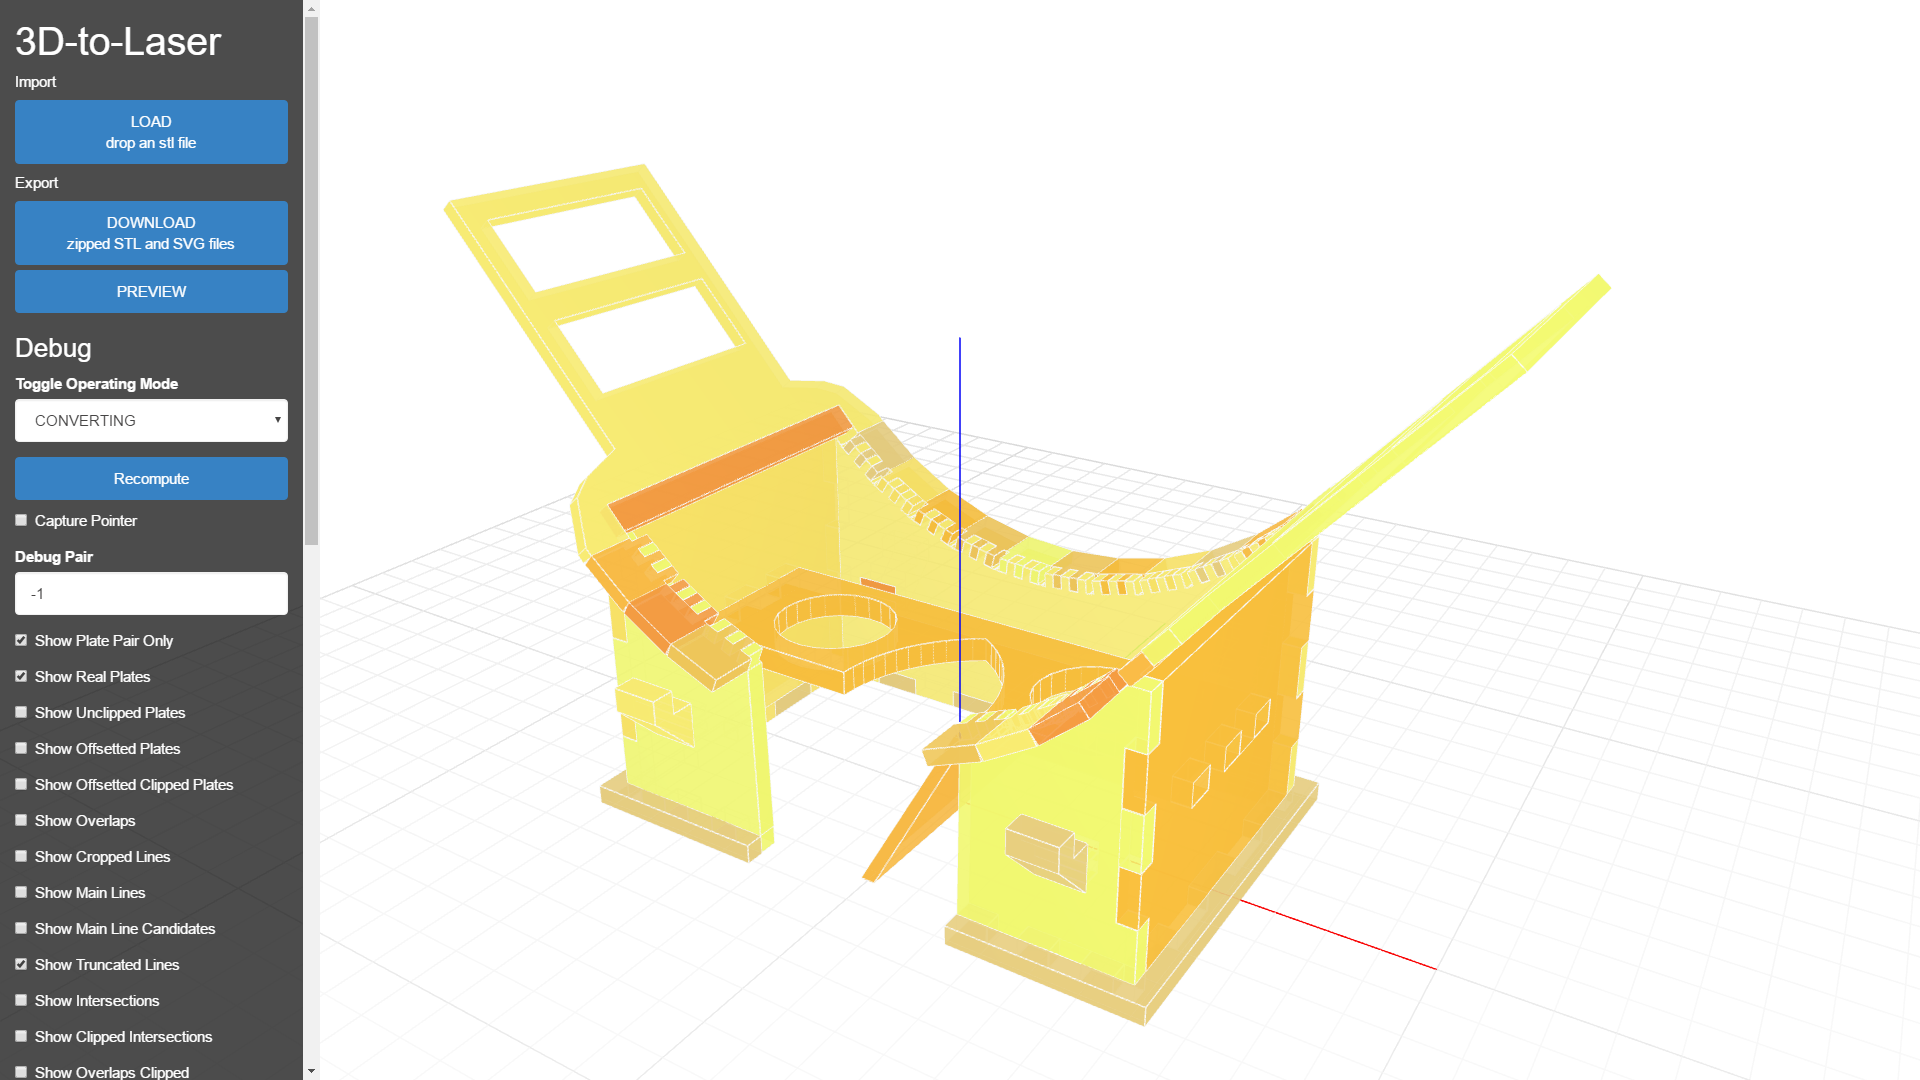
\includegraphics[width=1\columnwidth]{02-debug_view}
  \caption{The debug view for easier debugging of the pipeline and single steps.}
  \label{fig:debug_view}
\end{figure}

\subsection{Operating Mode for Testing the Pipeline or One Step}

We implemented two operation modes (see Figure~\ref{fig:operating_mode}).

\begin{figure}
  \centering
  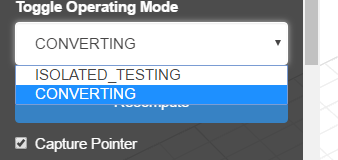
\includegraphics[width=0.5\columnwidth]{02-operating_mode}
  \caption{There are two different operation modes.}
  \label{fig:operating_mode}
\end{figure}

\subsubsection{Isolated\_testing for Single Step Debugging}

While \emph{Isolated\_testing} is selected there are only two additional options (see Figure~\ref{fig:isolated_testing}). The first is the step selection. With this the step that should be tested is selectable. The second is the \emph{testable} selection. This shows, depending on the selected step, test sets that could be used to test the step. Currently there are only for the steps  \emph{GeometryClassification} and  \emph{ClassifiedObjectsGraph} test sets available.

\begin{figure}
  \centering
  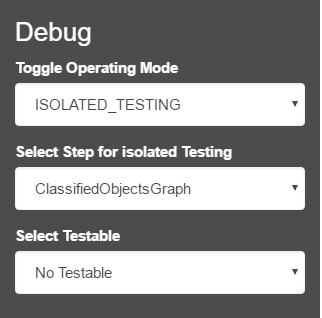
\includegraphics[width=0.5\columnwidth]{02-isolated_testing}
  \caption{There are two different operation modes.}
  \label{fig:isolated_testing}
\end{figure}

\subsubsection{Converting Enables Execution of Hole Pipeline}

If \emph{converting} is selected the hole pipeline is executed. A \threedmodel can be uploaded and is processed until the \svgfile{} is generated.

The \emph{Pipeline Methods} that are selectable are \emph{Stack Plates}, \emph{Find Plates} and \emph{Classifiers}.

For \emph{Stack Plate} and \emph{Classifiers} there are just the following additional options:

A radio button menu to change the rendering of the original model to hidden, solid, wireframe or just the vertices. A drop down offering multiple visualizer depending on the chosen operating mode and representing the corresponding pipeline steps. The test strip user interface to set the kerf for calibrating including the download button for the test strip.

In addition to these, while using the pipeline method \emph{Find Plates}, a field for setting the welding distance and several check box options are shown.

The following of those options effect only the \emph{PlateGraphVisualizer}: \emph{Show Plate Pair Only}, \emph{Show Real Plates}, \emph{Show Unclipped Plates}, \emph{Show Offset Plates}, \emph{Show Offset Clipped Plates}, \emph{Show Overlaps}, \emph{Show Cropped Lines}, \emph{Show Main Lines}, \emph{Show Main Line Candidates}, \emph{Show Truncated Lines}, \emph{Show Intersections}, \emph{Show Clipped Intersections} and \emph{Show Clipped Intersections}. The other effect only the \emph{FingerJointVisualizer}.

In both of these two visualizers the \emph{Capture Point} option can be used to click on a plate and get plate name and connection id's printed into the debugging console.

The option \emph{Platefinding Algorithm} offers the possibility to use only inherent plates for creating the plate graph and the following steps or using them with the extruded plates together.


%\subsection{Pipeline Visualizations}
% \subsection{Algorithm/ Method Selection}
% \subsection{Testables (Operating Mode)}
% \subsection{Console Debug Output}

\section{{\platener} as a Command Line Interface for Advanced Users}
\label{sec:walkthrough-cli}

We have seen in the preceding sections, how {\platener} is used in a
web browser.
% We intent to maximize scalability and user-friendliness
% by providing a web application.
Though converting a {\threedmodel} can be realized in a mere
drag-and-drop action using a web browser, we are limited to a single
conversion at a time. The web solution focuses on the results of the
conversion. Developers require a tool, that reports about the
conversion status and internal successful or failed processes. Our
software {\platener} provides a command line interface (CLI), which is
used in a terminal window. The CLI exposes commands for converting
{\threedmodel}s, processing multiple models in sequence and logging
progress reports. We explain the usage of the CLI in
Section~\sectionref{sec:walkthrough-cli-usage} and we demonstrate the logging
capabilities in Section~\sectionref{sec:walkthrough-cli-reports}.

\subsection{Usage Instructions of {\platener}'s CLI}
\label{sec:walkthrough-cli-usage}

A CLI is self-documenting. Listing~\ref{lst:cli-help} shows the
available commands.

\begin{listing}[!h]
\begin{minted}[
linenos
]{text}
node platener-cli.js -h

Specify an output directory.

  Usage: platener-cli [options] <output-dir>

  Options:

    -h, --help                output usage information
    -V, --version             output the version number
    -p --convertPath <input>  Convert multiple stl-Models to plates.
                              Give path to an folder with stl-Files.
    -f --convertFile <input>  Convert an stl-Model to plates.
                              Give path to an stl-File.
    -v --verbose              Enable Verbose Logging
    -s --subReports           Log Reports for each Fabrication Method
    --maxFilesize <input>     Limit filesize (MB),
                              so large files are skipped.

Full Help:

-f --convertFile    Generate all conversions for each
                    fabrication mode for the given stl-Model.
                    Each solution is stored in a seperate zip-File.
                    The zip-Files are written to the output directory.
\end{minted}
\caption{The help of {\platener}'s CLI.}
\label{lst:cli-help}
\end{listing}


The command line interface mirrors all the computational behavior of
{\platener} as a web application. With the CLI, we can convert a
single {\threedmodel} by loading data from the file system. The
conversion result is again a {\zipfile}. It is written to a given
target directory. We can recursively read input directories to
convert each {\stlfile} for the laser cutter. Both commands are given
in Listing~\ref{lst:cli-convert}.


\begin{listing}[!h]
\begin{minted}[
linenos
]{shell}
# convert a single file
node platener-cli.js -f ./stl/cubeFilled5cm.stl ./conversions

# convert an input directory
node platener-cli.js -f ./stl ./conversions
\end{minted}
\caption{Converting an {\stlfile} with {\platener}'s CLI.}
\label{lst:cli-convert}
\end{listing}

We can use the \emph{--maxFilesize} filter, to limit the
input files by their size in megabytes.

\subsection{Tracking Down Errors with Conversion Reports}
\label{sec:walkthrough-cli-reports}

Using the web application we either receive a successfully converted
{\svgfile} or the conversion fails. As the web interface is a
user-centered design we do not show extensive error messages or logs
of similar kind. For a developer it is crucial know where and under what
circumstances the software failed. With reports, we document the
conversion process. A report provides a short summary of the
conversion and gathers all error messages along the way, so a
developer can track down the issue. Figure~\ref{fig:report-simple}
shows a summary report. A report itemizing the results of our three
conversion approaches can be seen in Figure~\ref{fig:report-methods}.
In Figure~\ref{fig:report-error} an error message is depicted. When
multiple conversions were enqueued by {\platener}, we receive each
conversion report when the process finishes, as shown in
Figure~\ref{fig:report-multiple}.

\begin{figure}
  \centering
  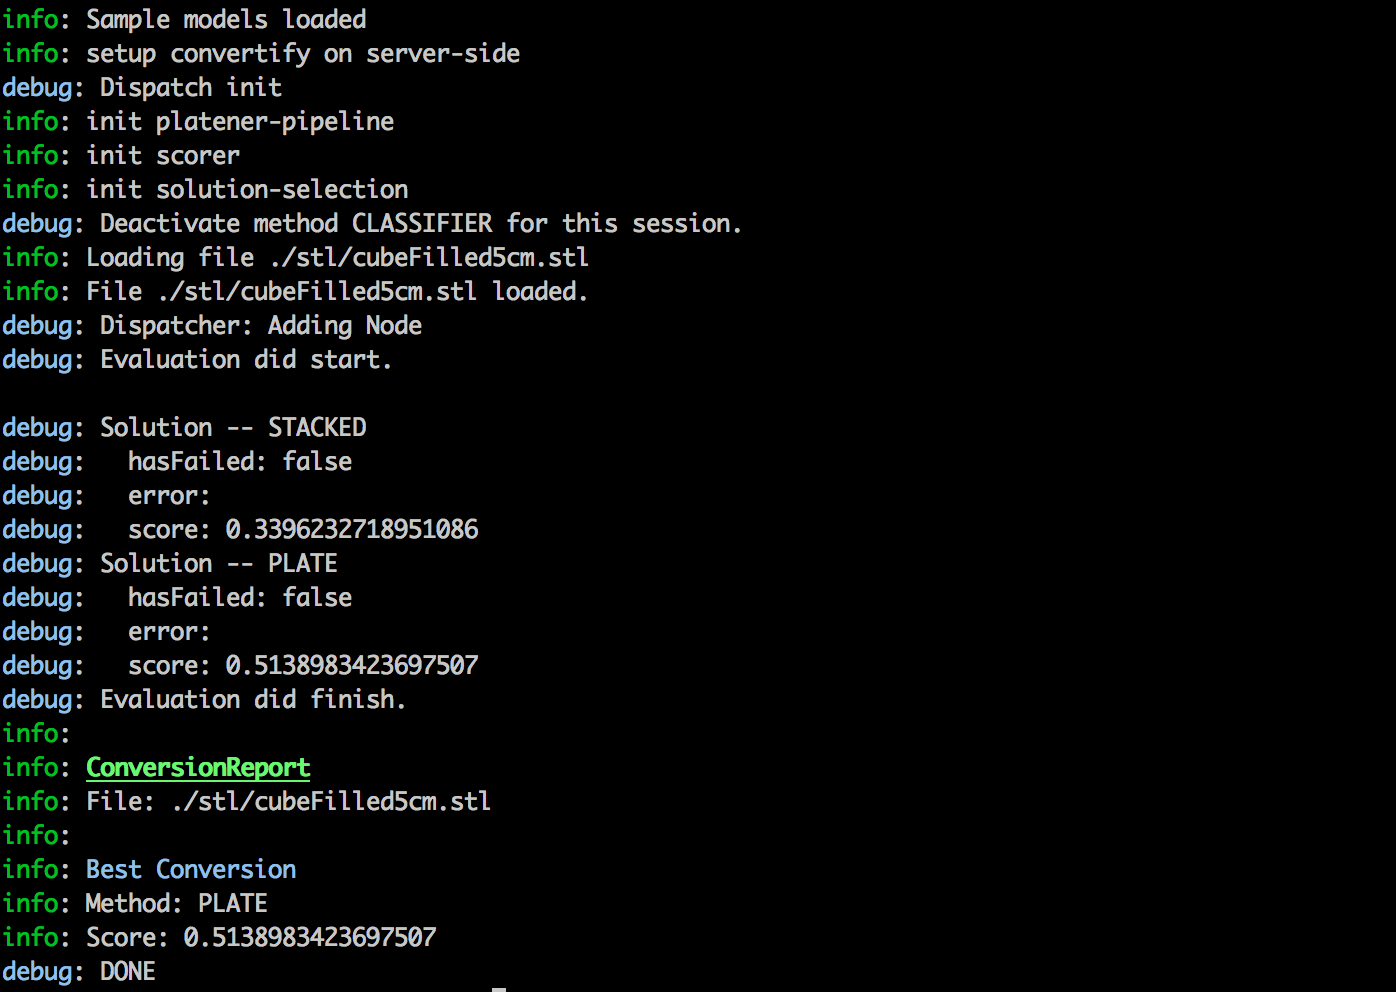
\includegraphics[width=1\columnwidth]{02-user-interaction-report-simple}
  \caption{A \class{Report}, showing a summary of the conversion.}
  \label{fig:report-simple}
\end{figure}

\begin{figure}
  \centering
  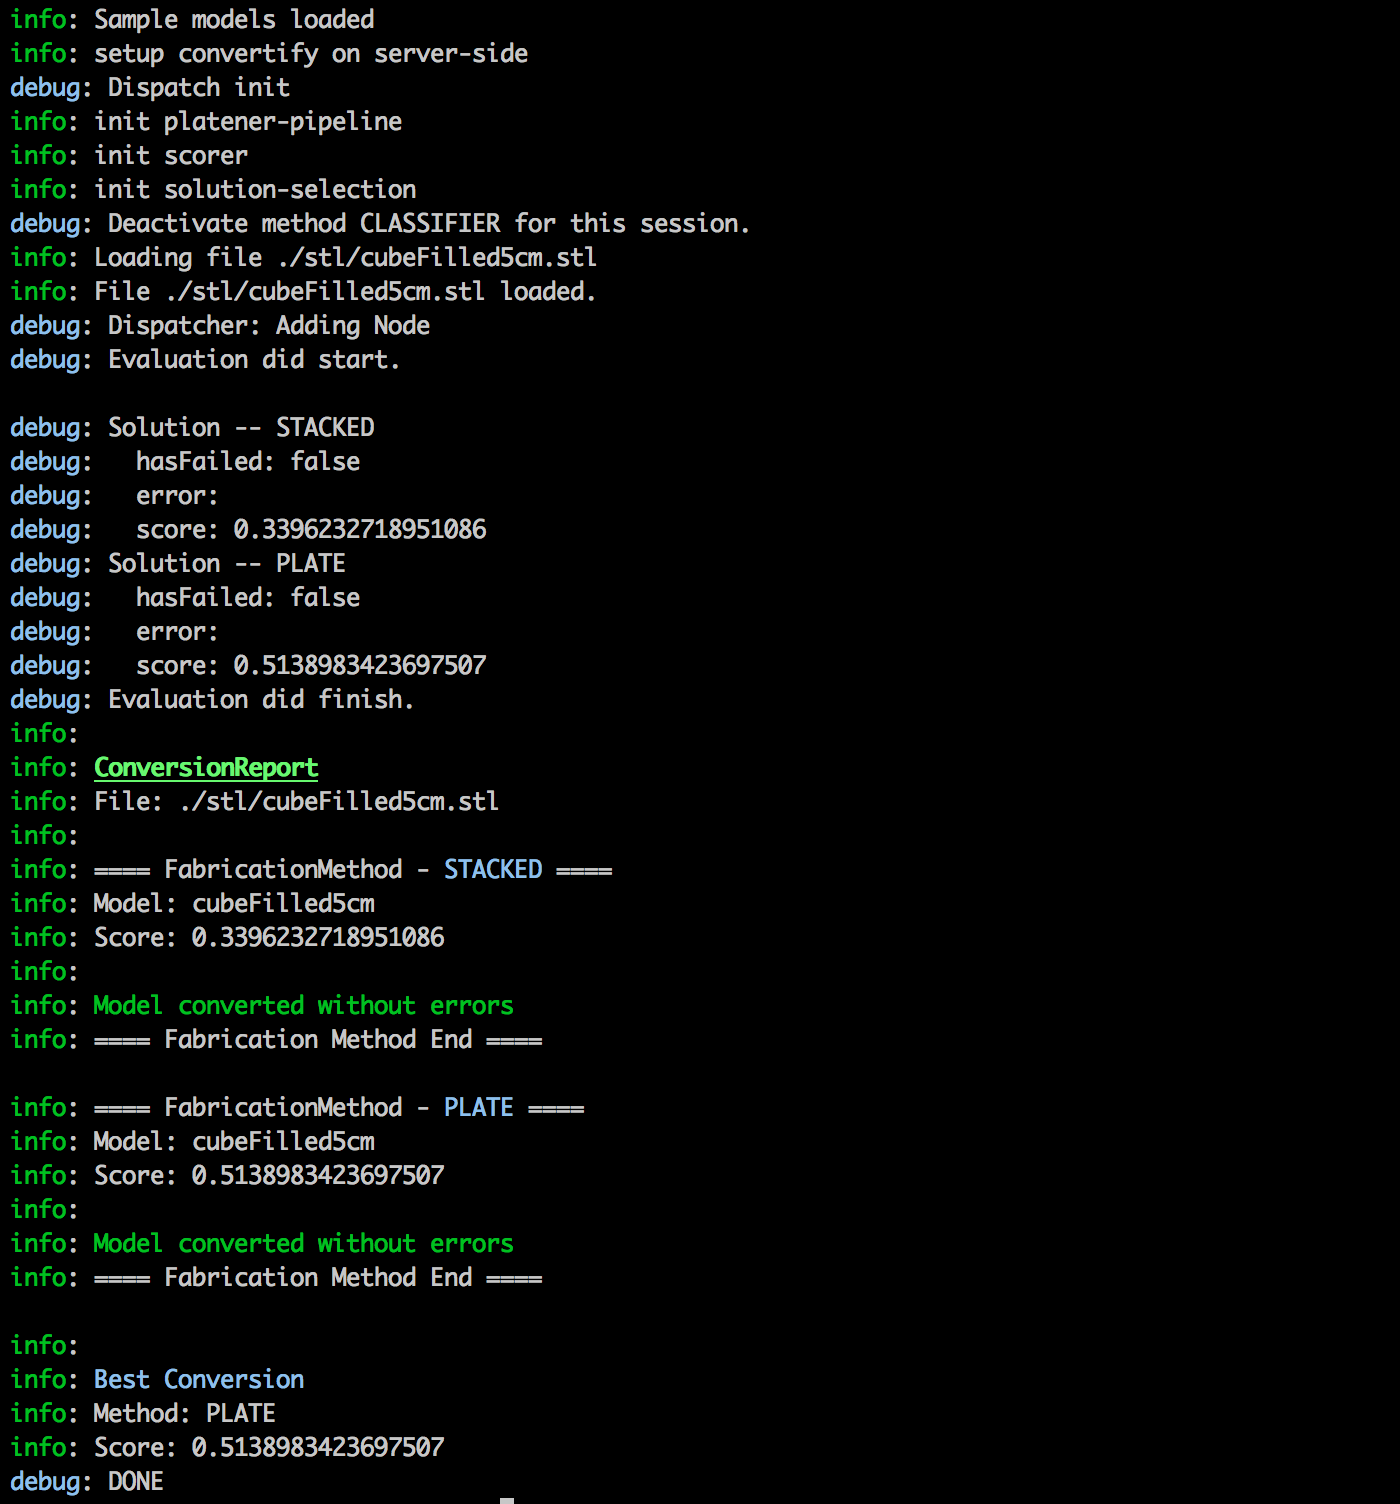
\includegraphics[width=1\columnwidth]{02-user-interaction-report-methods}
  \caption{A \class{Report}, showing a separate summary for each
    fabrication method of the conversion.}
  \label{fig:report-methods}
\end{figure}

\begin{figure}
  \centering
  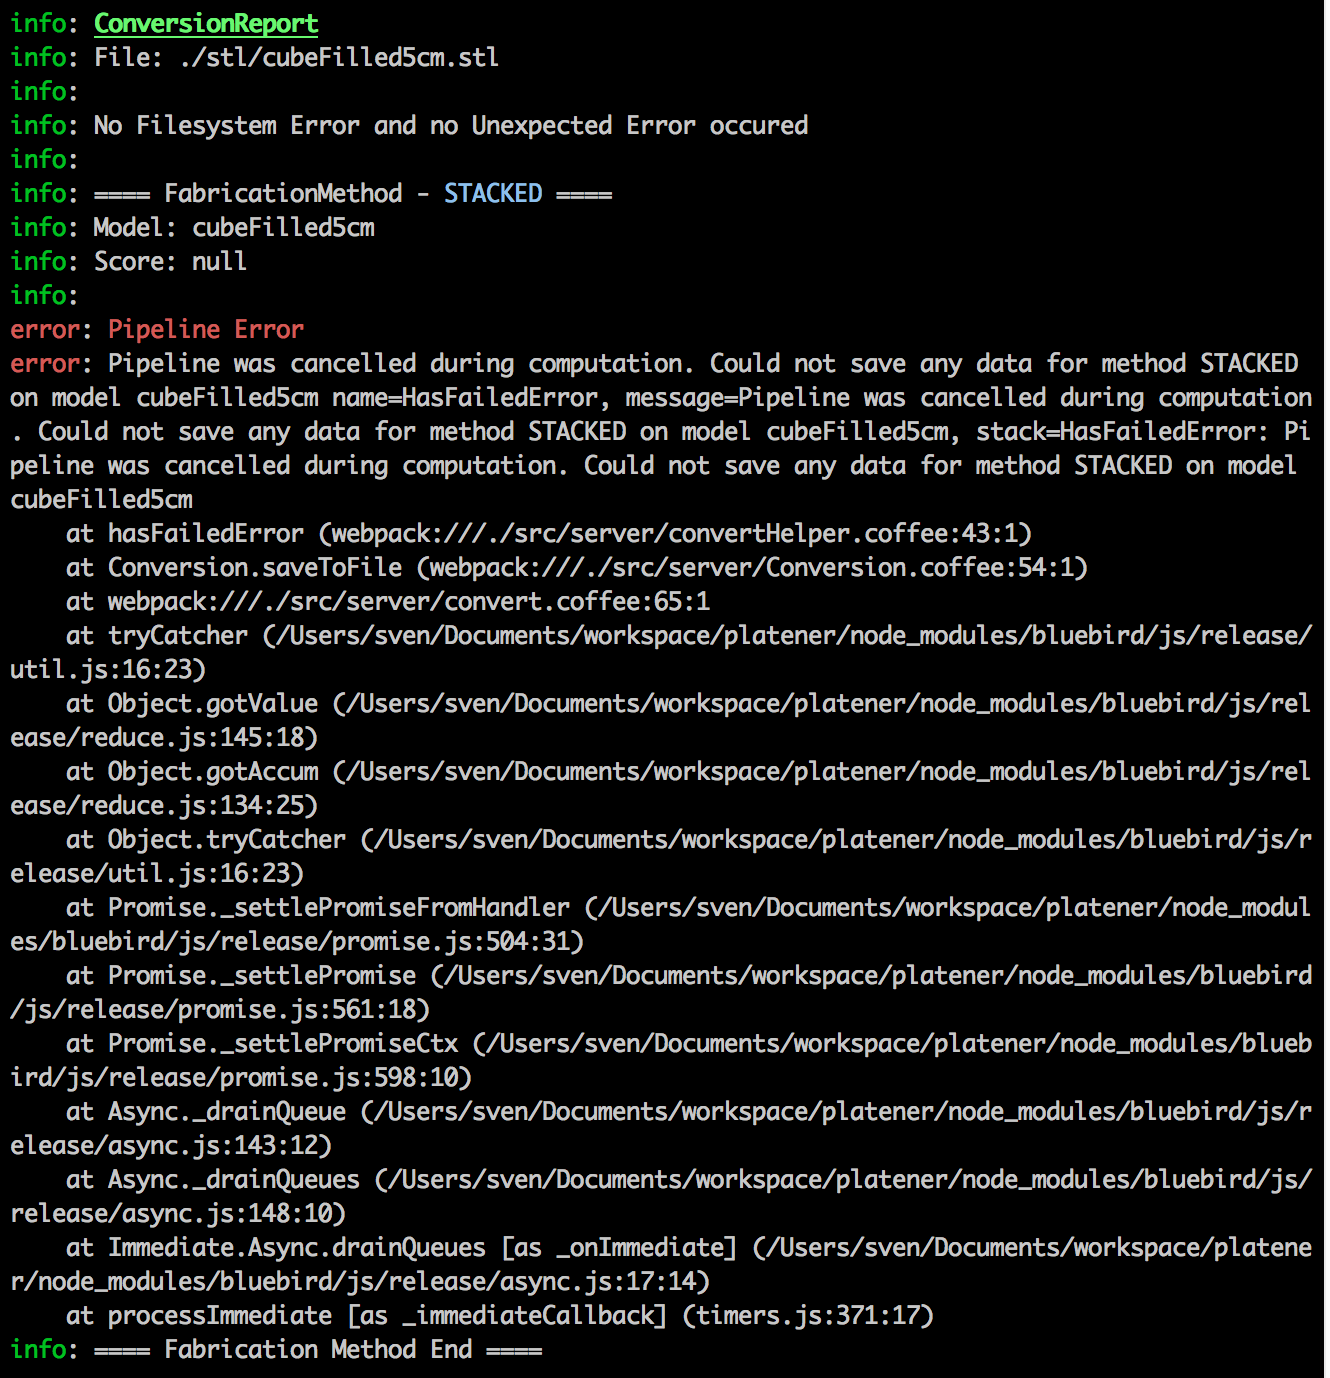
\includegraphics[width=0.8\columnwidth]{02-user-interaction-report-error}
  \caption{When a conversion fails the \class{Report} shows the error
    message.}
  \label{fig:report-error}
\end{figure}

\begin{figure}
  \centering
  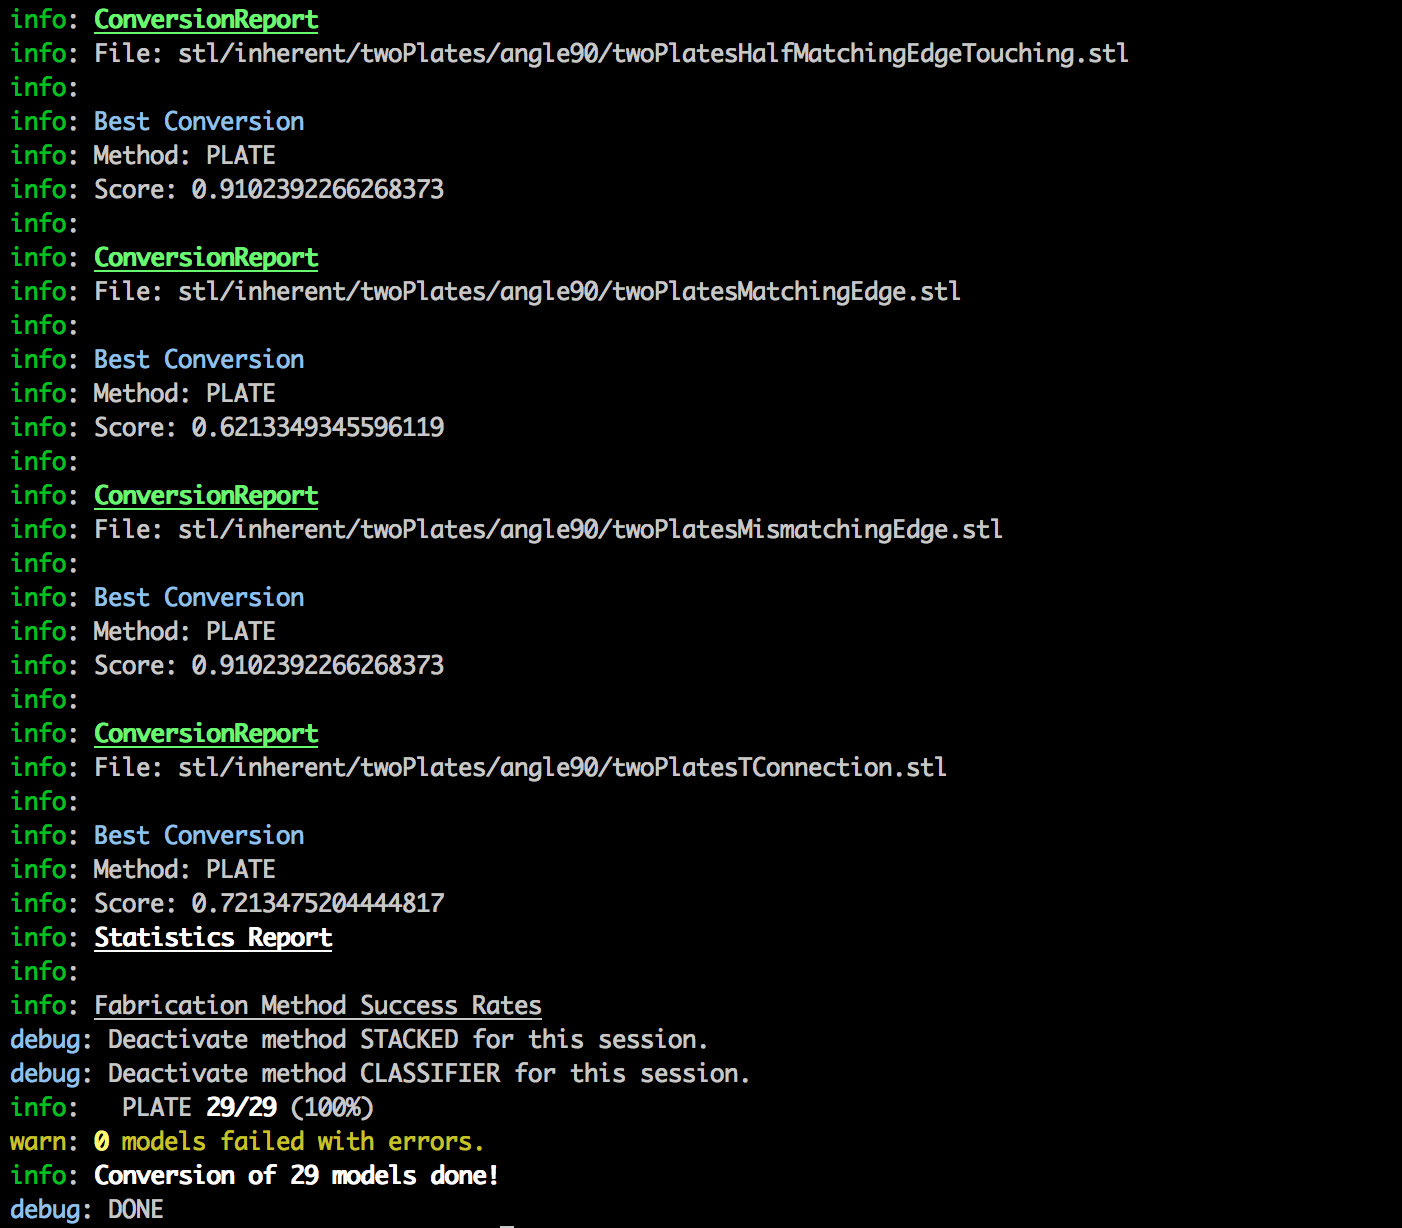
\includegraphics[width=0.8\columnwidth]{02-user-interaction-report-multiple}
  \caption{A sequence of conversions is summarized when the
    computation completed.}
  \label{fig:report-multiple}
\end{figure}



\end{document}

%%% Local Variables:
%%% mode: latex
%%% TeX-master: "../ClassicThesis"
%%% TeX-command-extra-options: "-shell-escape"
%%% End:
